%%%%%%%%%%%%%%%%%%%%%%%%%%%%%%%%%%%%%%%%%
% Beamer Presentation
% LaTeX Template
% Version 1.0 (10/11/12)
%
% This template has been downloaded from:
% http://www.LaTeXTemplates.com
%
% License:
% CC BY-NC-SA 3.0 (http://creativecommons.org/licenses/by-nc-sa/3.0/)
%
%%%%%%%%%%%%%%%%%%%%%%%%%%%%%%%%%%%%%%%%%

%----------------------------------------------------------------------------------------
%	PACKAGES AND THEMES
%----------------------------------------------------------------------------------------

\documentclass{beamer}

\mode<presentation> {

% The Beamer class comes with a number of default slide themes
% which change the colors and layouts of slides. Below this is a list
% of all the themes, uncomment each in turn to see what they look like.

%\usetheme{default}
%\usetheme{AnnArbor}
%\usetheme{Antibes}
%\usetheme{Bergen}
%\usetheme{Berkeley}
%\usetheme{Berlin}
%\usetheme{Boadilla}
%\usetheme{CambridgeUS}
%\usetheme{Copenhagen}
%\usetheme{Darmstadt}
%\usetheme{Dresden}
%\usetheme{Frankfurt}
%\usetheme{Goettingen}
%\usetheme{Hannover}
%\usetheme{Ilmenau}
%\usetheme{JuanLesPins}
%\usetheme{Luebeck}
\usetheme{Madrid}
%\usetheme{Malmoe}
%\usetheme{Marburg}
%\usetheme{Montpellier}
%\usetheme{PaloAlto}
%\usetheme{Pittsburgh}
%\usetheme{Rochester}
%\usetheme{Singapore}
%\usetheme{Szeged}
%\usetheme{Warsaw}

% As well as themes, the Beamer class has a number of color themes
% for any slide theme. Uncomment each of these in turn to see how it
% changes the colors of your current slide theme.

%\usecolortheme{albatross}
%\usecolortheme{beaver}
%\usecolortheme{beetle}
%\usecolortheme{crane}
%\usecolortheme{dolphin}
%\usecolortheme{dove}
%\usecolortheme{fly}
%\usecolortheme{lily}
%\usecolortheme{orchid}
%\usecolortheme{rose}
%\usecolortheme{seagull}
%\usecolortheme{seahorse}
%\usecolortheme{whale}
%\usecolortheme{wolverine}

%\setbeamertemplate{footline} % To remove the footer line in all slides uncomment this line
%\setbeamertemplate{footline}[page number] % To replace the footer line in all slides with a simple slide count uncomment this line

%\setbeamertemplate{navigation symbols}{} % To remove the navigation symbols from the bottom of all slides uncomment this line
}

\usepackage{graphicx} % Allows including images
\usepackage{booktabs} % Allows the use of \toprule, \midrule and \bottomrule in tables
\usepackage{amsmath} % Math env.
\usepackage{fontawesome} % Icons for GitHub, etc.

%----------------------------------------------------------------------------------------
%	TITLE PAGE
%----------------------------------------------------------------------------------------

\title[Kernel Learning]{Kernel Learning And Its Application In Nonlinear Support Vector Machines} % The short title appears at the bottom of every slide, the full title is only on the title page

\author{Anastasia S., Sven N., Joshua S.} % Your name
\institute[] % Your institution as it will appear on the bottom of every slide, may be shorthand to save space
{
Otto-Friedrich-University Bamberg \\ % Your institution for the title page
\medskip
\textit{anastasia.sinitsyna@stud.uni-bamberg.de \\}
\textit{sven-jason-waldemar.nekula@stud.uni-bamberg.de \\} % Your email address
\textit{joshua-guenter.simon@stud.uni-bamberg.de} % Your email address
}
\date{June 9, 2021} % Date, can be changed to a custom date

\begin{document}

\begin{frame}
\titlepage % Print the title page as the first slide
\end{frame}

\begin{frame}
\frametitle{Overview} % Table of contents slide, comment this block out to remove it
\tableofcontents % Throughout your presentation, if you choose to use \section{} and \subsection{} commands, these will automatically be printed on this slide as an overview of your presentation
\end{frame}


%----------------------------------------------------------------------------------------
%	PRESENTATION SLIDES
%----------------------------------------------------------------------------------------

%------------------------------------------------
\section{Introduction} 
%------------------------------------------------

\subsection{Linearly separable data classes}

\begin{frame}{}
    \frametitle{Linearly separable data classes}
    First, let's consider a given data set $\mathcal{X}$ of labeled points (inputs) with individual labels $y_i \in \left\{ -1,1 \right\}$, e.g. $(x_1,y_1), ..., (x_m, y_m) \in \mathcal{X} \times \left\{ -1,1 \right\}$. \\~\\
    
    Our goal is to implement a classification method, which is able to classify new and unlabeld data points with the right or "best" label. \\~\\
\end{frame}


\begin{frame}{}
	\frametitle{Linearly separable data classes}
	\begin{figure}
		\centering
		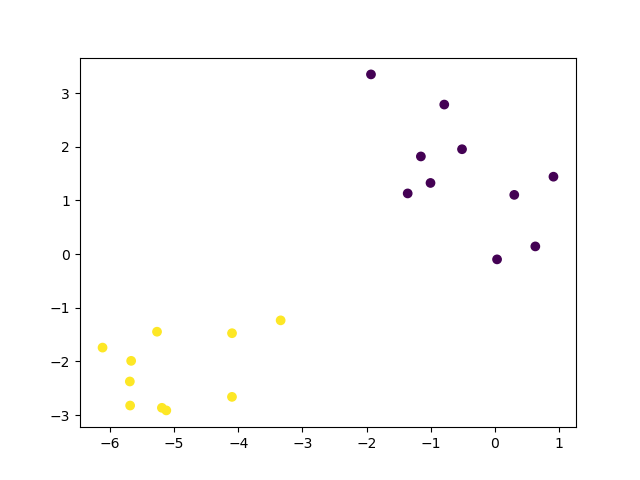
\includegraphics[width=0.7\linewidth]{img/LinearSVM_Data.png}
		\caption{ An example for linearly separable data.}
		\label{fig:lineardata}
	\end{figure} 
\end{frame}


\begin{frame}{}
    \frametitle{Linearly separable data classes}
    In machine learning, a well established classification method are the so called \textbf{Support Vector Machines} (SVM). Developed by Vladimir Vapnik and his coworkers in the 1990s, SVMs are still a relevent topic and an even more powerfull tool for \textbf{classification} and \textbf{regression}.
\end{frame}


%------------------------------------------------
\subsection{Similarity, dot product and vector norm}

\begin{frame}{}
    \frametitle{Similarity}
    To perform a classification, a similarity measure is needed. Finding a suitable measure is a core problem of machine learning. For now let's consider 
    \begin{equation}
        \begin{aligned}
            k: \mathcal{X} \times \mathcal{X} & \rightarrow \mathbb{R} \\
            (x, x') & \mapsto k(x, x')
        \end{aligned}
    \end{equation}
    where $k$ is a function that, given two patterns $x$ and $x'$, returns a real number characterizing their similarity. This function $k$ is called a \textbf{kernel}. Unless stated otherwise, $k(x, x') = k(x', x)$.
\end{frame}


\begin{frame}{}
    \frametitle{Dot product and vector norm}
    A simple type of similarity measure is a \textbf{dot product}. Given two vectors $x, x' \in \mathbb{R}^n$ the canonical dot product is defined as
    \begin{equation}
        \langle x,x' \rangle = (x')^T x = \sum_{i = 1}^{n} x_i x'_i.
    \end{equation}
    Futhermore this allows a calculation of the \textbf{norm} (length) of a single vector $x$ as 
    \begin{equation}
        \left\lVert x \right\rVert = \sqrt{\langle x,x \rangle}.
    \end{equation}
    More properties of vector spaces, dot products and norms can be found in \cite{Liesen}.
\end{frame}


%------------------------------------------------
\subsection{Hyperplane classifiers - Solving an optimization problem}

\begin{frame}{}
    \frametitle{Hyperplane classifiers}
    The underlying learning algorithm of SVMs yields to find a hyperplane in some dot product space $\mathcal{H}$, which separates the data. A hyperplane of the form
    \begin{equation}
        \langle w,x \rangle + b = 0
    \end{equation}
    where $w \in \mathcal{H}, b \in \mathbb{R}$ shall be considered \cite{Schoelkopf}(p. 11). Futhermore decision functions 
    \begin{equation}
        f(x) = sgn \left( \langle w,x \rangle + b \right)
    \end{equation}
    can be asigned.
\end{frame}


\begin{frame}{}
    \frametitle{Hyperplane classifiers - A constrained optimization problem}
    The \textbf{optimal hyperplane} can be calculated by finding the normal vector that leads to the largest margin. Thus we need to solve the optimization problem
    \begin{equation} \label{eq:1}
        \begin{aligned}
            \min_{w \in \mathcal{H}, b \in \mathbb{R}} \quad & \tau (w) = \frac{1}{2} \lVert w \rVert^2 \\
            \textrm{subject to} \quad & y_{i} \left( \langle w,x \rangle + b \right) \geq 1 \text{ } \forall i = {1, \dots, m}. 
        \end{aligned}
    \end{equation}
    The constraints in \eqref{eq:1} ensure that $f(x_i)$ will be $+1$ for $y_i = +1$ and $-1$ for  $y_i = -1$. The $\geq 1$ on the right hand side of the constraints effectively fixes the scaling of $w$. This leads to the maximum margin hyperplane. A detailed explanation can be found in \cite{Schoelkopf}(Chap 7).
\end{frame}


\begin{frame}{}
    \frametitle{Hyperplane classifiers - Lagrangian}
    The constrained optimization problem in \eqref{eq:1} can be re-written using the method of Lagrange multipliers. This leads to the Lagrangian
    \begin{equation} \label{eq:2}
        L(w,b,\alpha) = \frac{1}{2} \lVert w \rVert^2 - \sum_{i=1}^{m} \alpha_i \left( y_{i} \left( \langle w,x \rangle + b \right) - 1 \right)
    \end{equation}
    subject to $\alpha_i \geq 0 \text{ } \forall i = {1, \dots, m}$. Here, $\alpha_i$ are the Lagrange multipliers. The Lagrangian $L$ has to be minimized with respect to the primal variables $w$ and $b$ and maximized with respect to the dual variables $\alpha_i$ (in other words, a saddle point has to be found).
\end{frame}


\begin{frame}{}
    \frametitle{Hyperplane classifiers - KKT conditions}
    The Karush-Kuhn-Tucker (KKT) complementarity conditions of optimization theory state, that at the saddle point, the derivatives of $L$ with respect to the
    primal variables must vanish, since
    \begin{equation}
        \frac{\partial}{\partial b} L(w,b,\alpha) = 0 \text{ and } \frac{\partial}{\partial w} L(w,b,\alpha) = 0
    \end{equation}
    leads to
    \begin{equation} \label{eq:3}
        \sum_{i=1}^{m} \alpha_i y_i = 0 \text{ and } w = \sum_{i=1}^{m} \alpha_i y_i x_i.
    \end{equation}
    The solution vector $w$ thus has an expansion in terms of a subset of the training patterns, namely those patterns with non-zero $\alpha_i$, called Support Vectors (SVs).
\end{frame}


\begin{frame}{}
    \frametitle{Hyperplane classifiers - Dual optimization problem}
    We can again re-write our optimization problem by substituting \eqref{eq:3} into the Lagrangian \eqref{eq:2} to eliminate the primal variables. This yields the dual optimization problem, which is usually solved in practice
    \begin{equation} \label{eq:4}
        \begin{aligned}
            \max_{\alpha \in \mathbb{R}^m} \quad & W(\alpha) = \sum_{i=1}^{m} \alpha_i - \frac{1}{2} \sum_{i,j=1}^{m} \alpha_i \alpha_j y_i y_j \langle x_i,x_j \rangle \\
            \textrm{subject to} \quad & \alpha_i \geq 0 \text{ } \forall i = {1, \dots, m} \text{ and } \sum_{i=1}^{m} \alpha_i y_i = 0. 
        \end{aligned}
    \end{equation}
\end{frame}


\begin{frame}{}
    \frametitle{Hyperplane classifiers - Dual optimization problem}
    Finally, the decision function can be re-written using \eqref{eq:3} as
    \begin{equation} \label{eq:5}
        f(x) = sgn \left( \sum_{i=1}^{m} \alpha_i y_i \langle x,x_i \rangle + b \right),
    \end{equation}
    where $b$ can be computed by exploiting $\alpha_i \left[ y_i \left( \langle x_i,w \rangle + b \right) - 1 \right] = 0$, which follows from the KKT conditions. \\~\\
    Details on mathematical optimization and convex constrained problems can be found in \cite{Jarre}. Explanations on dealing with nonlinear problems are given in \cite{Reinhardt}.
\end{frame}



%------------------------------------------------
\section{Linear SVMs}
%------------------------------------------------

\subsection{Maximum margin separator}

\begin{frame}{}
    \frametitle{Maximum margin separator}
    We now have all the theoretical background to go back to our inital classification problem. We can implement a SVM as a maximum margin separator for the given data set $\mathcal{X}$. \\~\\  
\end{frame}


\begin{frame}{}
	\frametitle{Maximum margin separator}
	\begin{figure}
		\centering
		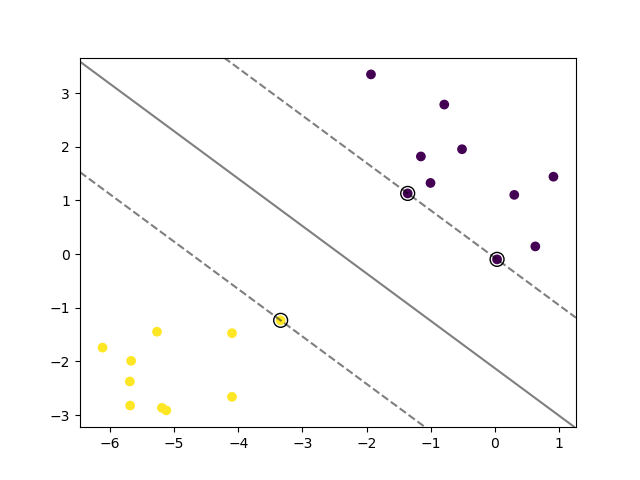
\includegraphics[width=0.7\linewidth]{img/LinearSVM_complete.png}
		\caption{Implementation of a SVM using the 'linear' Kernel.}
		\label{fig:linearsvm}
	\end{figure}
	 
\end{frame}


%------------------------------------------------
\subsection{Limitations}

\begin{frame}{}
	\frametitle{Limitations}
	Let's consider the following data set. \\~\\ 
	\begin{figure}
		\centering
		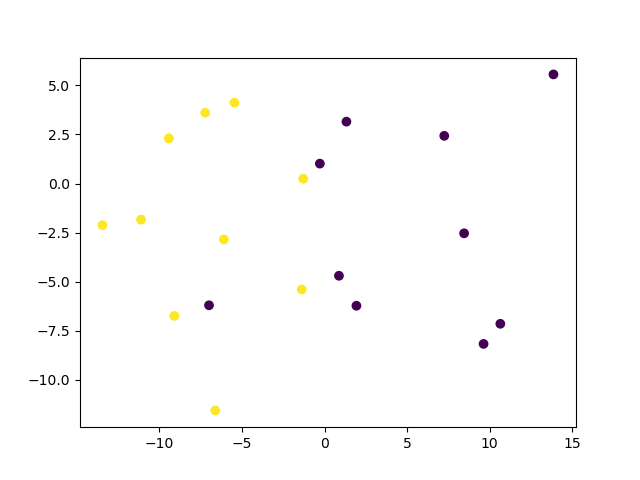
\includegraphics[width=0.7\linewidth]{img/SlackData}
		\caption{Linearly or separable or not?}
		\label{fig:slackdata}
	\end{figure}
\end{frame}

\begin{frame}{}
	\frametitle{Soft Margin Hyperplanes}
	We introduce a slack variable
	\begin{equation}
		\xi_{ i } \geq 0 \text{ } \forall i = {1, \dots, m}
	\end{equation}
	in the simplest case, this leads to 
	\begin{equation}
		\begin{aligned}
			\min_{w \in \mathcal{H}, \xi \in \mathbb{R}^{n}} \quad & \tau (w, \xi) = \frac{1}{2} \lVert w \rVert^2 + \frac{C}{m} \sum_{i=1}^{m} \xi_{i} \\
			\textrm{subject to} \quad & y_{i} \left( \langle w,x \rangle + b \right) \geq 1 - \xi_{i} \text{ } \forall i = {1, \dots, m}, 
		\end{aligned}
	\end{equation}
    where $C \in \mathbb{R}$ is a regularization parameter.
\end{frame}


\begin{frame}{}
	\frametitle{Soft Margin Hyperplanes}
	Our dual optimization problem also gets rewritten as
    \begin{equation} \label{eq:7}
        \begin{aligned}
            \max_{\alpha \in \mathbb{R}^m} \quad & W(\alpha) = \sum_{i=1}^{m} \alpha_i - \frac{1}{2} \sum_{i,j=1}^{m} \alpha_i \alpha_j y_i y_j \langle x_i,x_j \rangle \\
            \textrm{subject to} \quad & 0 \leq \alpha_i \leq \frac{C}{m} \text{ } \forall i = {1, \dots, m} \text{ and } \sum_{i=1}^{m} \alpha_i y_i = 0. 
        \end{aligned}
	\end{equation}
	This classifier is referred to as C-SV classifier and can be used to prevent overfittintg by allowing the classifier to make false classifications. \\
	More classifiers using soft margins can be found in \cite{Schoelkopf}(Chap. 7.5).
\end{frame}


\begin{frame}{}
	\frametitle{Soft Margin Hyperplanes}
	\begin{figure}
		%\centering
		%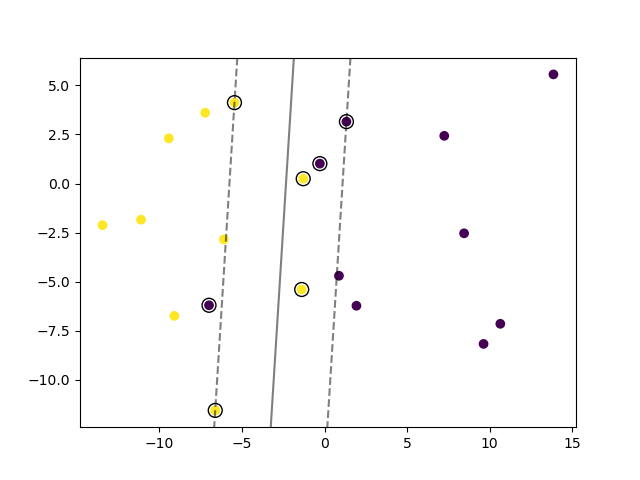
\includegraphics[width=0.7\linewidth]{img/SlackSVM}
        \begin{tabular}{ll}
    		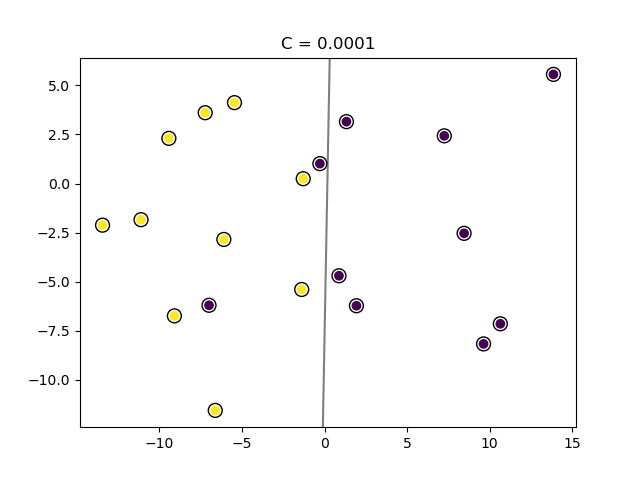
\includegraphics[scale=0.25]{img/SlackSVM01.png}
    		&
    		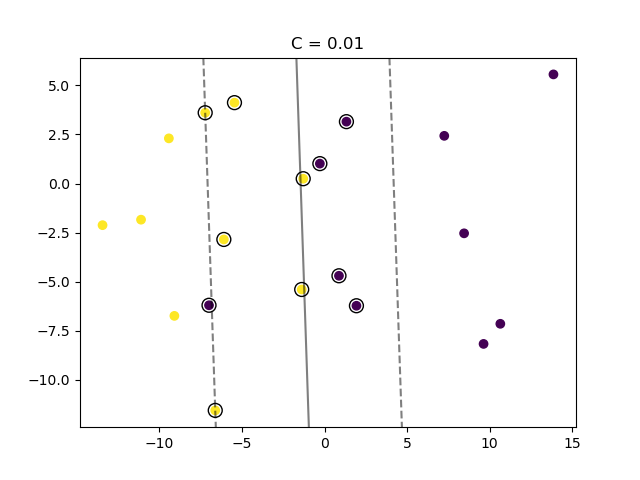
\includegraphics[scale=0.25]{img/SlackSVM02.png} \\
            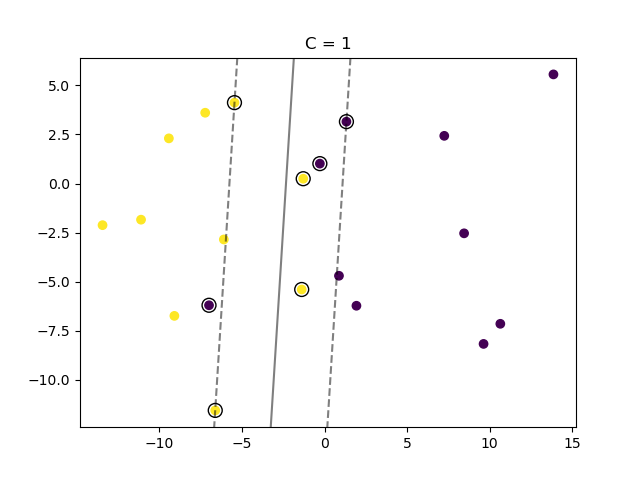
\includegraphics[scale=0.25]{img/SlackSVM03.png}
    		&
    		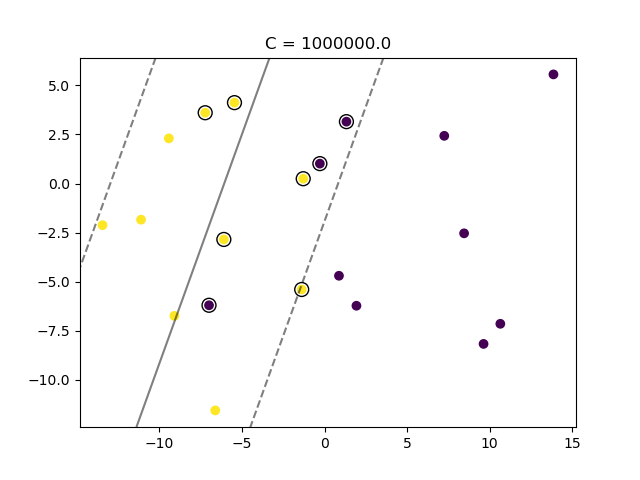
\includegraphics[scale=0.25]{img/SlackSVM04.png}
    	\end{tabular}
		\caption{Implementation of a SVM using the 'linear' Kernel different soft margins.}
		\label{fig:slacksvm}
	\end{figure}
\end{frame}


\begin{frame}{}
    \frametitle{Limitations}
    Let's consider the following data sets. \\~\\ 
    \begin{figure}[h]
    	\begin{tabular}{ll}
    		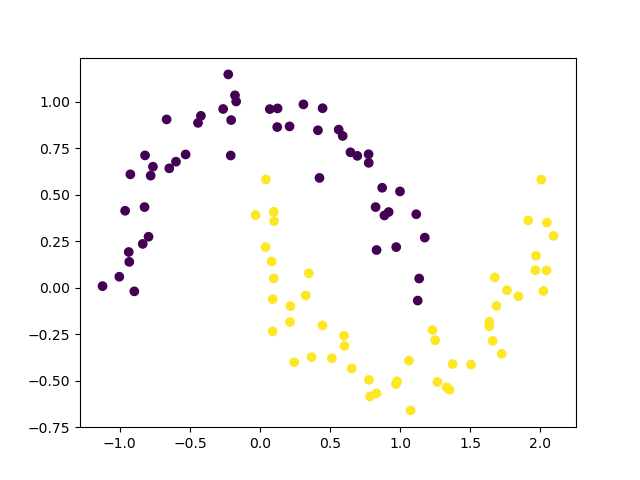
\includegraphics[scale=0.35]{img/moonshape.png}
    		&
    		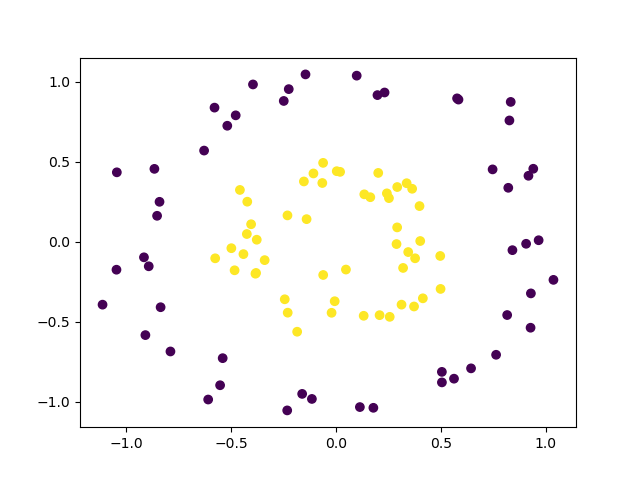
\includegraphics[scale=0.35]{img/circleshape.png}
    	\end{tabular}
    	\caption{Two examples of data that can't be linearly separated.}
    	\label{Fig:nonlineardata}
    \end{figure}
\end{frame}


\begin{frame}{}
	\frametitle{Limitations}
	What happens if you try to seperate them linearly? \\~\\ 
	\begin{figure}[h]
		\begin{tabular}{ll}
			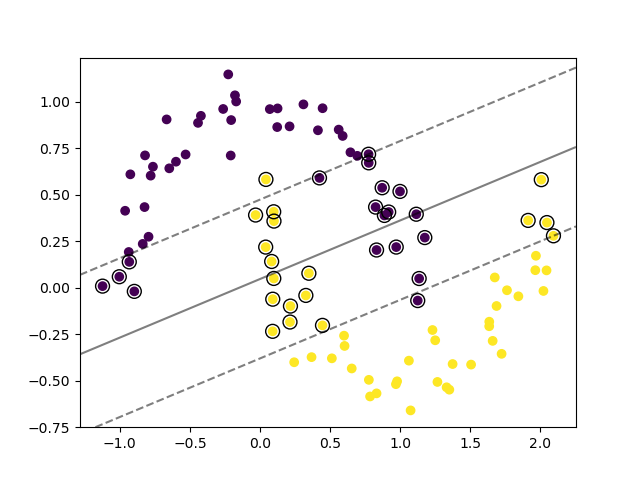
\includegraphics[scale=0.35]{img/linearSVM_moon.png}
			&
			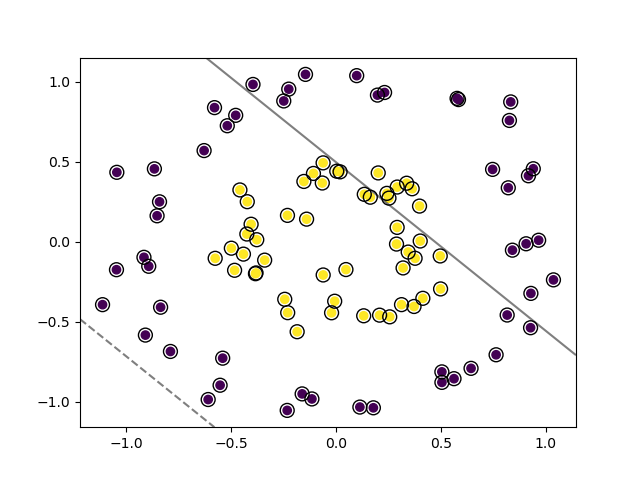
\includegraphics[scale=0.35]{img/linearSVM_circles.png}
		\end{tabular}
		\caption{SVMs using the 'linear' Kernel.}
		\label{Fig:nlinearsvmnonlineardata}
	\end{figure}
\end{frame}



%------------------------------------------------
\section{Nonlinear SVMs}
%------------------------------------------------

\subsection{The kernel trick}

\begin{frame}{}
	\frametitle{The kernel trick}
	To extend the introduced SVM algorithm, we can substitut \eqref{eq:5} by applying a kernel of the form
    \begin{equation}
        k(x,x') = \langle \Phi (x), \Phi (x_i) \rangle
    \end{equation}
    where 
    \begin{equation}
        \begin{aligned}
            \Phi: \mathcal{X} & \rightarrow \mathcal{H} \\
            (x) & \mapsto \Phi (x)
        \end{aligned}
    \end{equation}
    is a function that maps an input from $ \mathcal{X} $ to a dot product space $ \mathcal{H} $. This is referred to as the \textbf{kernel trick}.
\end{frame}


\begin{frame}{}
	\frametitle{The kernel trick}
	We then obtain decision functions of the form
    \begin{align}
        f(x) & = sgn \left( \sum_{i=1}^{m} \alpha_i y_i \langle \Phi (x), \Phi (x_i) \rangle + b \right) \\ 
        & = sgn \left( \sum_{i=1}^{m} \alpha_i y_i k(x,x_i) + b \right)
    \end{align}
    and the optimization problem
    \begin{equation} \label{eq:6}
        \begin{aligned}
            \max_{\alpha \in \mathbb{R}^m} \quad & W(\alpha) = \sum_{i=1}^{m} \alpha_i - \frac{1}{2} \sum_{i,j=1}^{m} \alpha_i \alpha_j y_i y_j k(x, x_i) \\
            \textrm{subject to} \quad & \alpha_i \geq 0 \text{ } \forall i = {1, \dots, m} \text{ and } \sum_{i=1}^{m} \alpha_i y_i = 0. 
        \end{aligned}
    \end{equation}
\end{frame}


\begin{frame}{}
	\frametitle{The kernel trick}
    The $m \times m$ Matrix $K$ with elements $K_{ij} = k(x_i, x_j)$ is called the \textbf{Gram matrix} (or kernel matrix) of $k$. \\~\\
    A kernel $k$ is called \textbf{positive definite kernel}, when the Gram matrix $K$ is positive definite. \\~\\
	As stated in \cite{Schoelkopf}(Chap. 2): \textit{Given an algorithm which is formulated in terms of a positive definite kernel $k$, one can construct an alternative algorithm by replacing $k$ by another positive definite kernel $\tilde{k}$.}
\end{frame}


\begin{frame}{}
	\frametitle{The kernel trick}
	The kernel trick can be applied since all feature vectors only occurred in dot products. A more precise explanation can be found in \cite{Schoelkopf}(Chap. 2).
\end{frame}


%------------------------------------------------
\subsection{Solving non linearly separable classification problems}

\begin{frame}{}
	\frametitle{A suitable kernel}
	Going back to our problem of non linearly separable data, we can use a kernel function of the form
    \begin{equation}
        k(x, x') = \exp \left( - \frac{\left\lVert x - x' \right\rVert^2}{2 \sigma^2} \right),
    \end{equation}
    a so called \textbf{Gaussian radial basis function} (GRBF or RBF kernels) with $ \sigma > 0$.
\end{frame}


\begin{frame}{}
	\frametitle{Solving the nonlinear problem}
	\begin{figure}[h]
		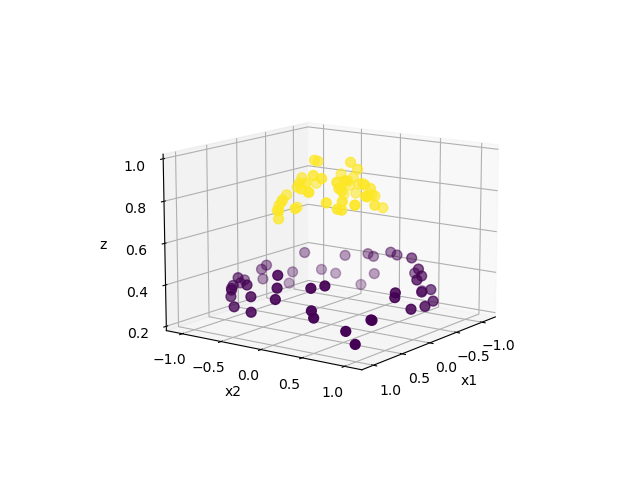
\includegraphics[scale=0.5]{img/Circle3D.png}
		\caption{Data points mapped to a 3-dimensional space using the 'rbf' kernel.}
		\label{Fig:rbf3d}
	\end{figure}
\end{frame}


\begin{frame}{}
	\frametitle{Solving the nonlinear problem}
	\begin{figure}[h]
		\begin{tabular}{ll}
			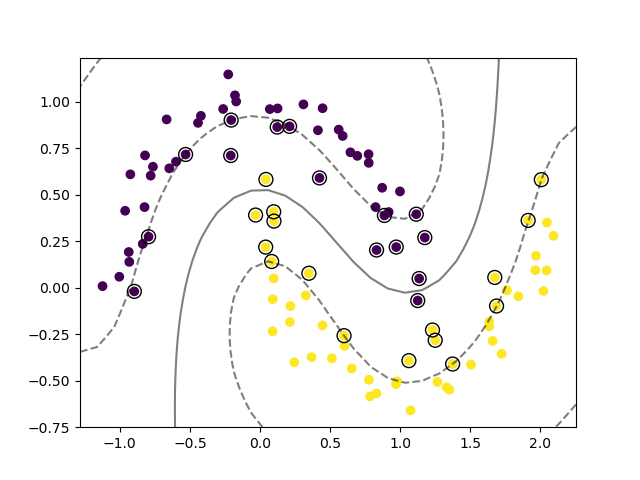
\includegraphics[scale=0.35]{img/rbfSVM_moon.png}
			&
			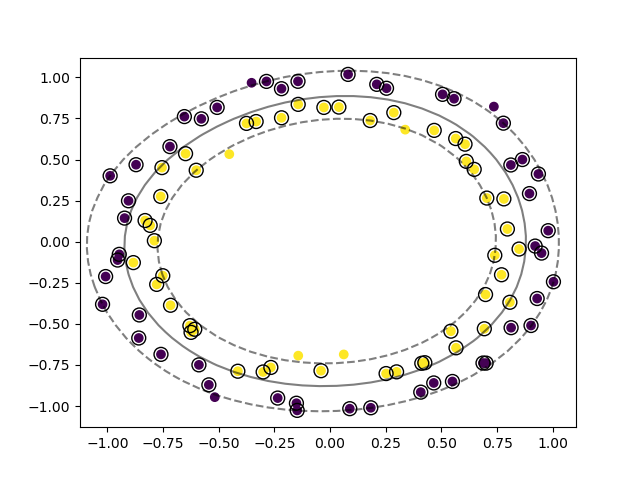
\includegraphics[scale=0.35]{img/rbfSVM_circles.png}
		\end{tabular}
		\caption{SVMs using the 'rbf' Kernel.}
		\label{Fig:rbfsvms}
	\end{figure}
\end{frame}


%------------------------------------------------
\subsection{A closer look at kernels}

\begin{frame}{}
	\frametitle{Examples of kernels}
    An overview of common kernels:
    \begin{itemize}
        \item \textbf{Linear}: $k(x,x') = \langle x, x' \rangle$
        \item \textbf{Polynomial}: $k(x,x') = \langle x, x' \rangle^{d}, d \in \mathbb{N}$
        \item \textbf{Inhomogeneous Polynomial}: $k(x,x') = \left( \langle x, x' \rangle + c \right)^{d}, d \in \mathbb{N}, c \geq 0$
        \item \textbf{Gaussian}: $k(x, x') = \exp \left( - \frac{\left\lVert x - x' \right\rVert^2}{2 \sigma^2} \right), \sigma > 0$
        \item \textbf{Sigmoid}: $k(x, x') = \tanh \left( \kappa \langle x, x' \rangle + \vartheta \right), \kappa > 0, \vartheta < 0$
    \end{itemize}
    \bigskip
    These kernels are implemented in the Python modul scikit-learn \texttt{sklearn.svm} based on the libsvm implementation in C\texttt{++} by Chih-Chung Chang and Chih-Jen Lin \cite{libsvm}.
\end{frame}

%------------------------------------------------



%------------------------------------------------
\section{More kernel applications}

\begin{frame}{}
	\frametitle{More kernel applications}
    Some interessting kernel applications:
    \begin{itemize}
        \item Image recognition/classification (with SVMs)
        \item Computer vision and computer graphics, 3D reconstruction
        \item Kernel principal component analysis
    \end{itemize}
\end{frame}
%------------------------------------------------



%------------------------------------------------
% References
%------------------------------------------------

\begin{frame}
    \frametitle{References}
    \footnotesize{
        \begin{thebibliography}{99} % Beamer does not support BibTeX so references must be inserted manually as below
            \bibitem[Schölkopf, 2002]{Schoelkopf} Schölkopf, Bernhard, Alexander J. Smola
            \newblock Learning with Kernels: Support Vector Machines, Regularization, Optimization, and Beyond. MIT press, 2002.

            \bibitem[Liesen, 2015]{Liesen} Liesen, Jörg, Volker Mehrmann
            \newblock Lineare Algebra. Wiesbaden, Germany: Springer, 2015.

            \bibitem[Jarre, 2019]{Jarre} Jarre, Florian, Josef Stoer
            \newblock Optimierung: Einführung in mathematische Theorie und Methoden. Springer-Verlag, 2019.

            \bibitem[Reinhardt, 2012]{Reinhardt} Reinhardt, Rüdiger, Armin Hoffmann, Tobias Gerlach
            \newblock Nichtlineare Optimierung: Theorie, Numerik und Experimente. Springer-Verlag, 2012.

            \bibitem[Chang, 2011]{libsvm} Chang, Chih-Chung, Chih-Jen Lin
            \newblock LIBSVM : A library for support vector machines. ACM Transactions on Intelligent Systems and Technology, 2:27:1--27:27, 2011. Software available at \url{https://www.csie.ntu.edu.tw/~cjlin/libsvm/}.

            % Example entry.
            %\bibitem[Smith, 2012]{p3} John Smith (2002)
            %\newblock Title of the publication
            %\newblock \emph{Journal Name} 12(3), 45 -- 678.
        \end{thebibliography}
    }
\end{frame}

%------------------------------------------------

\begin{frame}
    \Huge{\centerline{Time for your questions!}}
    \bigskip
    \bigskip
    \bigskip
    \bigskip

    \normalsize
    Follow our development on GitHub \faicon{github} 
    \url{https://github.com/JoshuaSimon/Kernel-Learning}
    
\end{frame}

%----------------------------------------------------------------------------------------

\end{document} 